\let\negmedspace\undefined
\let\negthickspace\undefined
%\RequirePackage{amsmath}
\documentclass[journal,12pt,twocolumn]{IEEEtran}
 \usepackage{gensymb}
%\doublespacing
 \usepackage{polynom}
%\singlespacing
%\usepackage{silence}
%Disable all warnings issued by latex starting with "You have..."
%\usepackage{graphicx}
\usepackage{amssymb}
%\usepackage{relsize}
\usepackage[cmex10]{amsmath}
%\usepackage{amsthm}
%\interdisplaylinepenalty=2500
%\savesymbol{iint}
%\usepackage{txfonts}
%\restoresymbol{TXF}{iint}
%\usepackage{wasysym}
\usepackage{amsthm}
%\usepackage{pifont}
%\usepackage{iithtlc}
% \usepackage{mathrsfs}
% \usepackage{txfonts}
 \usepackage{stfloats}
% \usepackage{steinmetz}
 \usepackage{bm}
% \usepackage{cite}
% \usepackage{cases}
% \usepackage{subfig}
%\usepackage{xtab}
\usepackage{longtable}
%\usepackage{multirow}
%\usepackage{algorithm}
%\usepackage{algpseudocode}
\usepackage{enumitem}
 \usepackage{mathtools}
 \usepackage{tikz}
% \usepackage{circuitikz}
% \usepackage{verbatim}
%\usepackage{tfrupee}
\usepackage[breaklinks=true]{hyperref}
%\usepackage{stmaryrd}
%\usepackage{tkz-euclide} % loads  TikZ and tkz-base
%\usetkzobj{all}
\usepackage{listings}
    \usepackage{color}                                            %%
    \usepackage{array}                                            %%
    \usepackage{longtable}                                        %%
    \usepackage{calc}                                             %%
    \usepackage{multirow}                                         %%
    \usepackage{hhline}                                           %%
    \usepackage{ifthen}                                           %%
  %optionally (for landscape tables embedded in another document): %%
    \usepackage{lscape}     
% \usepackage{multicol}
% \usepackage{chngcntr}
%\usepackage{enumerate}
\usepackage{tfrupee}

%\usepackage{wasysym}
%\newcounter{MYtempeqncnt}
\DeclareMathOperator*{\Res}{Res}
\DeclareMathOperator*{\equals}{=}
%\renewcommand{\baselinestretch}{2}
%\renewcommand\thesection{\arabic{section}}
%\renewcommand\thesubsection{\thesection.\arabic{subsection}}
%\renewcommand\thesubsubsection{\thesubsection.\arabic{subsubsection}}

%\renewcommand\thesectiondis{\arabic{section}}
%\renewcommand\thesubsectiondis{\thesectiondis.\arabic{subsection}}
%\renewcommand\thesubsubsectiondis{\thesubsectiondis.\arabic{subsubsection}}

% correct bad hyphenation here
\hyphenation{op-tical net-works semi-conduc-tor}
\def\inputGnumericTable{}                                 %%

\lstset{
frame=single, 
breaklines=true,
columns=fullflexible
}
\newtheorem{theorem}{Theorem}[section]
\newtheorem{problem}{Problem}
\newtheorem{proposition}{Proposition}[section]
\newtheorem{lemma}{Lemma}[section]
\newtheorem{corollary}[theorem]{Corollary}
\newtheorem{example}{Example}[section]
\newtheorem{definition}[problem]{Definition}
%\newtheorem{thm}{Theorem}[section] 
%\newtheorem{defn}[thm]{Definition}
%\newtheorem{algorithm}{Algorithm}[section]
%\newtheorem{cor}{Corollary}
\newcommand{\BEQA}{\begin{eqnarray}}
\newcommand{\EEQA}{\end{eqnarray}}
\newcommand{\define}{\stackrel{\triangle}{=}}
\newcommand*\circled[1]{\tikz[baseline=(char.base)]{
    \node[shape=circle,draw,inner sep=2pt] (char) {#1};}}
\bibliographystyle{IEEEtran}
%\bibliographystyle{ieeetr}
\providecommand{\mbf}{\mathbf}
\providecommand{\pr}[1]{\ensuremath{\Pr\left(#1\right)}}
\providecommand{\qfunc}[1]{\ensuremath{Q\left(#1\right)}}
\providecommand{\sbrak}[1]{\ensuremath{{}\left[#1\right]}}
\providecommand{\lsbrak}[1]{\ensuremath{{}\left[#1\right.}}
\providecommand{\rsbrak}[1]{\ensuremath{{}\left.#1\right]}}
\providecommand{\brak}[1]{\ensuremath{\left(#1\right)}}
\providecommand{\lbrak}[1]{\ensuremath{\left(#1\right.}}
\providecommand{\rbrak}[1]{\ensuremath{\left.#1\right)}}
\providecommand{\cbrak}[1]{\ensuremath{\left\{#1\right\}}}
\providecommand{\lcbrak}[1]{\ensuremath{\left\{#1\right.}}
\providecommand{\rcbrak}[1]{\ensuremath{\left.#1\right\}}}
\theoremstyle{remark}
\newtheorem{rem}{Remark}
\newcommand{\sgn}{\mathop{\mathrm{sgn}}}
\providecommand{\fourier}{\overset{\mathcal{F}}{ \rightleftharpoons}}
%\providecommand{\hilbert}{\overset{\mathcal{H}}{ \rightleftharpoons}}
\providecommand{\system}{\overset{\mathcal{H}}{ \longleftrightarrow}}
	%\newcommand{\solution}[2]{\textbf{Solution:}{#1}}
\newcommand{\solution}{\noindent \textbf{Solution: }}
\newcommand{\cosec}{\,\text{cosec}\,}
\providecommand{\dec}[2]{\ensuremath{\overset{#1}{\underset{#2}{\gtrless}}}}
\newcommand{\myvec}[1]{\ensuremath{\begin{pmatrix}#1\end{pmatrix}}}
\newcommand{\mydet}[1]{\ensuremath{\begin{vmatrix}#1\end{vmatrix}}}
%\numberwithin{equation}{section}
%\numberwithin{figure}{section}
%\numberwithin{table}{section}
%\numberwithin{equation}{subsection}
%\numberwithin{problem}{section}
%\numberwithin{definition}{section}
\makeatletter
\@addtoreset{figure}{problem}
\makeatother
\let\StandardTheFigure\thefigure
\let\vec\mathbf
%\renewcommand{\thefigure}{\theproblem.\arabic{figure}}
%\renewcommand{\thefigure}{\theproblem}
%\setlist[enumerate,1]{before=\renewcommand\theequation{\theenumi.\arabic{equation}}
%\counterwithin{equation}{enumi}
%\renewcommand{\theequation}{\arabic{subsection}.\arabic{equation}}
\def\putbox#1#2#3{\makebox[0in][l]{\makebox[#1][l]{}\raisebox{\baselineskip}[0in][0in]{\raisebox{#2}[0in][0in]{#3}}}}
     \def\rightbox#1{\makebox[0in][r]{#1}}
     \def\centbox#1{\makebox[0in]{#1}}
     \def\topbox#1{\raisebox{-\baselineskip}[0in][0in]{#1}}
     \def\midbox#1{\raisebox{-0.5\baselineskip}[0in][0in]{#1}}
\title{Assignment 2}
\author{ Vedant Bhandare (cs21btech11007)}

\begin{document}

\maketitle
\begin{abstract}
This document contains the solution for Assignment 2 (ICSE Class 12 Maths 2019 Q.18)
\end{abstract}
\begin{flushleft}
\textbf{Q18 [ICSE 12 2019]:}Draw a sketch and find the area bounded by the curve $x^2 = y$ and $x + y = 2$
\textbf{Solution: } The given parabola $x^2 - y = 0$ can written in vector form as
\begin{align}
    \vec{x}^T\vec{a}\vec{x} + \vec{b}^T\vec{x} + \vec{c} = 0
\end{align}
with the parameters,
\begin{align}
    \vec{a} = \myvec{1 & 0 \\ 0 & 0}, \vec{b} = \myvec{0 \\ -1}, \vec{c} = 0
\end{align}
The line $x + y = 2$ can be written as
\begin{align}
    \vec{x} = \vec{p} + \lambda \vec{m}
\end{align}
where $\vec{p}$ is a point and $\vec{m}$ is the direction vector of the line\\
Choosing $\vec{p}$ as $\myvec{1 \\ 1}$, we get:
\begin{align}
    \vec{x} = \myvec{1 \\ 1} + \lambda \myvec{1 \\ -1}
\end{align}
The intersection of this line with the parabola is given by
\begin{align}
    \vec{x_i} = \myvec{1 \\ 1} + \lambda_i \myvec{1 \\ -1}
\end{align}
where $\lambda_i$ is given by,
\begin{multline}
\footnotesize
    \lambda_i = \frac{1}
{
\vec{m}^T\vec{a}\vec{m}
}
\lbrak{-\vec{m}^T\brak{\vec{a}\vec{p}+\vec{b}}}
\\
\pm
\rbrak{\sqrt{\sbrak{\vec{m}^T\brak{\vec{a}\vec{p}+\vec{b}}
}^2
-
\brak
{
\vec{p}^T\vec{a}\vec{p} + 2\vec{u}^T\vec{p} +c
}
\brak{\vec{m}^T\vec{a}\vec{m}}
}
}
\label{eq:tangent_roots}
\end{multline}
Substituting the values in above equation, we get
\begin{align}
    \lambda_i = 0, -3
\end{align}
Using these values of $\lambda$, the intersection points are,
\begin{align}
    \myvec{-2 \\ 4} \text{and} \myvec{1 \\ 1}
\end{align}

\vfill\null 
\columnbreak

From the figure below, the required area is equal to,
\begin{align}
    \text{Area of trapezium ABCD - Area under the parabola}
\end{align}
\begin{multline}
    = \frac{1}{2}\times (4 + 1)\times 3 - \int_{-2}^{1} x^2 dx = 7.5 - \sbrak{\frac{x^3}{3}}_{-2}^1 \\
    = \text{\fbox{4.5} sq.units \hspace{2.4cm}}
\end{multline}
The blue shaded region in the figure below represents this area.
\begin{figure}[ht]
    \centering
    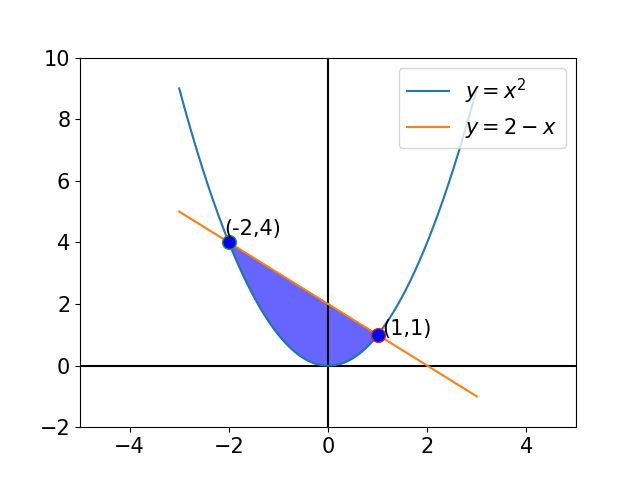
\includegraphics[width = \columnwidth]{Figures/Figure.png}
    \caption{Plot of line and parabola}
    \label{Figure}
\end{figure}
\end{flushleft}
\end{document}
